% !TeX root = ../main.tex
% Add the above to each chapter to make compiling the PDF easier in some editors.

\chapter{Introduction}\label{chapter:introduction}

Cyber security education is in high demand in any field which has critical responsibilities such as managing energy systems, monitoring airplanes, hospital management and in many other places.Recent incidents in Cyber security field shows that attackers are targeting vital points of a country or a city. According to CSIS\footnote{Center for Strategic & International Studies}, twelve crucial cyber attacks, to different countries around the world in June 2022, for instance one of them is targeted Lithuania's public infrastructures such as state railways, airports.\cite{cyberincidents} Indiviuals are target of cyber crime, today, everyone receives a millions of dollars from their distanced relatives with a mail to click. Surprisingly this phishing technique is still used and it works even though, not at targeted rate. 

% To have precautions against cyber attacks or attempts of them, self-awareness and interest of persons should be increased about cyber security. Recent developments in the world, forced people to have faster digitization of learning. COVID-19 pandemic proved that almost anything related to computers can be done online. Lectures, conferences, consultation by doctors and more moved to online sessions. However, as usage of internet increased and is going to be increased more in the future, cyber security became as much as crucial compared to previous years. 

In this paper, an open source virtualised security education platform, named Haaukins, will be discussed in depth and its working mechanism will be investigated in detail. The main aim of the platform to increase self awareness of people about cyber security and provide practical challenges to the participants. The platform does not require any preliminary information and includes variety of challenges at different levels.
Initially, the platform is built for high-school students to have very basic and simple access to cyber security challenges.Since existing platforms usually require virtual private network (VPN) to access virtualised environment, which brings overhead for high school students. Additionally, the platform itself is completely open source and can be deployed to any Debian based machines at universities, institutions, high schools or even individual local computer. In time, Haaukins proved its success in Denmark, then advanced challenges are included for experienced users. The management of the platform was not at good condition due to the fact that administrators of the platform should install command line tool to manage the platform. As the platform usage increased and spread through universities, management of the platform should be easier and no one should require to install any tool to manage the platform. Therefore, administrator side as well as challenges inside the platform developed according to feedback received from users of the platform. The platform includes practical exercises which are in the format of Jeopardry Capture-The-Flag(CTF).\cite{191767} The format is also being used by other security education platforms  such as Hackthebox\footnote{https://www.hackthebox.com}, picoCTF\footnote{https://picoctf.org}. Main idea is to have a secret string, called 'flag', in a virtualized vulnerable environment and participants of the game should exploit the vulnerability to receive value of  the 'flag'. The challenges in Haaukins platform is developed parallel to curricula of educational institutions. The content of the challenges in the platform shaped by lecture contents at universities or high schools, to consolidate theoretical information with real life practice. 
% Cheating at platform is still possible however compared to other existing platforms, it is difficult. Since Hauukins platform has unique flags to same questions which prevents participants to copy and paste the flags.







% Use with pdfLaTeX and Biber.

% \section{Section}
% Citation test (with Biber)~\parencite{latex}.

% \subsection{Subsection}

% See~\autoref{tab:sample}, \autoref{fig:sample-drawing}, \autoref{fig:sample-plot}, \autoref{fig:sample-listing}, \autoref{fig:tum}, \autoref{fig:tumslide}.

% \begin{table}[htpb]
%   \caption[Example table]{An example for a simple table.}\label{tab:sample}
%   \centering
%   \begin{tabular}{l l l l}
%     \toprule
%       A & B & C & D \\
%     \midrule
%       1 & 2 & 1 & 2 \\
%       2 & 3 & 2 & 3 \\
%     \bottomrule
%   \end{tabular}
% \end{table}

% \begin{figure}[htpb]
%   \centering
%   % This should probably go into a file in figures/
%   \begin{tikzpicture}[node distance=3cm]
%     \node (R0) {$R_1$};
%     \node (R1) [right of=R0] {$R_2$};
%     \node (R2) [below of=R1] {$R_4$};
%     \node (R3) [below of=R0] {$R_3$};
%     \node (R4) [right of=R1] {$R_5$};

%     \path[every node]
%       (R0) edge (R1)
%       (R0) edge (R3)
%       (R3) edge (R2)
%       (R2) edge (R1)
%       (R1) edge (R4);
%   \end{tikzpicture}
%   \caption[Example drawing]{An example for a simple drawing.}\label{fig:sample-drawing}
% \end{figure}

% \begin{figure}[htpb]
%   \centering

%   \pgfplotstableset{col sep=&, row sep=\\}
%   % This should probably go into a file in data/
%   \pgfplotstableread{
%     a & b    \\
%     1 & 1000 \\
%     2 & 1500 \\
%     3 & 1600 \\
%   }\exampleA
%   \pgfplotstableread{
%     a & b    \\
%     1 & 1200 \\
%     2 & 800 \\
%     3 & 1400 \\
%   }\exampleB
%   % This should probably go into a file in figures/
%   \begin{tikzpicture}
%     \begin{axis}[
%         ymin=0,
%         legend style={legend pos=south east},
%         grid,
%         thick,
%         ylabel=Y,
%         xlabel=X
%       ]
%       \addplot table[x=a, y=b]{\exampleA};
%       \addlegendentry{Example A};
%       \addplot table[x=a, y=b]{\exampleB};
%       \addlegendentry{Example B};
%     \end{axis}
%   \end{tikzpicture}
%   \caption[Example plot]{An example for a simple plot.}\label{fig:sample-plot}
% \end{figure}

% \begin{figure}[htpb]
%   \centering
%   \begin{tabular}{c}
%   \begin{lstlisting}[language=SQL]
%     SELECT * FROM tbl WHERE tbl.str = "str"
%   \end{lstlisting}
%   \end{tabular}
%   \caption[Example listing]{An example for a source code listing.}\label{fig:sample-listing}
% \end{figure}

% \begin{figure}[htpb]
%   \centering
%   
\includegraphics[width=0.8\textwidth]{tum}
%   \caption[Something else can be written here for listing this, otherwise the caption will be written!]{Includegraphics searches for the filename without extension first in logos, then in figures.} \label{fig:tum}
% \end{figure}

% \begin{figure}[htpb]
%   \centering
%   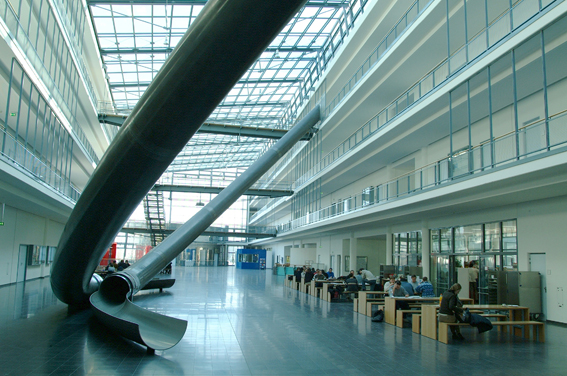
\includegraphics[width=0.8\textwidth]{figures/tum}
%   \caption{For pictures with the same name, the direct folder needs to be chosen.} \label{fig:tumslide}
% \end{figure}

% \begin{figure}[!tbp]
%   \centering
%   \subfloat[TUM Logo][The logo.]{
\includegraphics[height=0.2\textheight]{tum}\label{fig:tum1}}
%   \hfill
%   \subfloat[TUM Slide][The famous slide.]{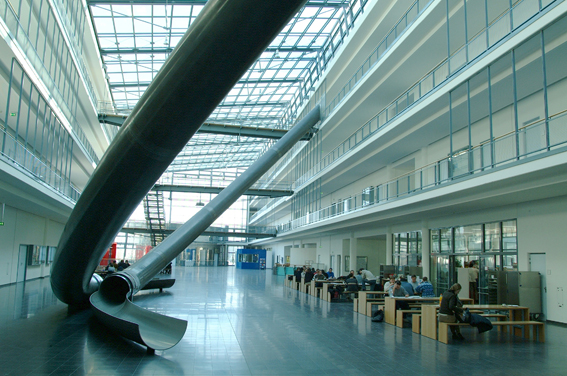
\includegraphics[height=0.2\textheight]{figures/tum}\label{fig:tum2}}
%   \caption{Two TUM pictures side by side.}
%   \label{fig:sidebyside}
% \end{figure}

% This is how the glossary will be used.

% \Glspl{ddye}, \gls{r0}, \gls{R0}, and \gls{kdeac}. Also, the \glspl{tum} has many \glspl{computer}, not only one \Gls{computer}. Subsequent acronym usage will only print the short version of \glspl{tuma} (take care of plural, if needed!), like here with \gls{tuma}, too. It can also be --> \glsdisp{tum}{hidden}\footnote{Example for a hidden TUM glossary entry.} <--.

% \todo{Now it is your turn to write your thesis.

% This will be a few tough weeks.}

% \done{Nevertheless, celebrate it when it is done!}
